% ---------------------------------------------------------
\chapter{Background and Related Work}
\label{b_rel_work}
% ---------------------------------------------------------

This chapter provides fundamental concepts of this thesis. 
In section~\ref{background} an introduction about variability models, performance assessment and performance prediction is given. 
Related work and approaches that analyse performance similar to our approach are summarized in section~\ref{rel_work}.

\section{Background}
\label{background}

The background section provides an introduction about necessary fundamentals. 
We give an overview about configurable software systems~(section~\ref{background_conf_sys}) and variability models~(section~\ref{background_variab_models}). 
We define the term performance~(section~\ref{background_perf}) for this thesis, describe how performance of software can be measured and how to learn models in order to be able to predict performance.

\subsection{Configurable Software Systems}
\label{background_conf_sys}
% Problem Space (Whole space) - Constraints (illegal feature combinations), default settings, optimizations, ... -> Solution Space ()
% variability models of configurable software systems
Today, almost every software system provides different options to configure them. 
Each combination of configurations results in a \textit{variant} of the program, similar to \acp{SPL}\footnote{``A \ac{SPL} is a set of software-intensive systems that share a common, managed set of features satisfying the specific needs of a particular market segment or mission which are developed from a common set of core assets in a prescribed way.''~\cite{northrop2010spl}}~\cite{siegmund2012spl}. 
Each variant comprises the set of activated configuration options, which are referred to as \textit{features}. 
The combination of features describe the user desired characteristics of the program~\cite{czarnecki2000generative}.
For Database Management Systems, the selection (or rejection) of features like compression, encryption or the use of a specific indexing strategy results in a number of different variants that fulfil different requirements desired by users. 
\todo{Functional - non-functional properties clarification}
Requirements that describe what a system can do are called functional properties~\cite{siegmund2012spl,guo2013variability}. 
In addition to the functionality requirements of software, there are also non-functional properties to be met~\cite{siegmund2012spl,guo2013variability,sarkar2015cost,siegmund2015performance}.
\todo{own words for quotes}
In literature, there exist different definitions of non-functional properties. 
Glinz surveyed the existing definitions in 2007~\cite{glinz2007non}, e.g. ``The required overall attributes of the system, including portability, reliability, efficiency, human engineering, testability, understandability, and modifiability''~\cite{davis1993software} or ``Requirements which are not specifically concerned with the functionality of a system. 
They place restrictions on the product being developed and the development process, and they specify external constraints that the product must meet''~\cite{kotonya1998requirements}. 
There are more definitions of non-functional properties, but in this thesis we want to adapt to the definition of Robertson and Robertson from 1999 because these definition has been widely used since its publication (used by:~\cite{nuseibeh2000requirements,jackson2001problem,cohn2004user,siegmund2012spl}): ``A property, or quality, that the product must have, such as an appearance, or a speed or accuracy property''~\cite{robertson1999mastering}.

\subsection{Variability Models}
\label{background_variab_models}

After defining configurable software systems with their functional and non-functional properties, we want to show how to model them. 
\textit{Feature models} define a common way to describe all valid configurations of software systems~\cite{siegmund2015performance,sarkar2015cost,guo2013variability}. 
They were introduced in 1990 by Kang et al.~\cite{kang1990feature} and since have became an important instrument for modelling variability in software product lines. 
With feature models, every configuration option can be expressed as a feature. 
There are two different representations of feature models: textual notations and graphical representations. 
Feature models in textual from (like SXFM~\cite{Mendonca2009SSP} and Velvet~\cite{rosenmuller2011multi}) have been developed to construct and maintain models of systems with a huge amount of features which might be presented poorly with a graphical tool. 
Whereas feature models with a graphical representation (also called feature diagrams~\cite{kang1990feature}) provide the possibility to create and manipulate feature models through a graphical user interface. 
Furthermore, feature diagrams are widely used in scientific literature to present analysed systems. 


Feature diagrams build up a tree-structured graph, as can be seen in the example diagram shown in figure~\ref{background_variab_models_feature_diagram_example}. 
With this example diagram, we will describe the elements of feature diagrams. 
The root node of the tree \textsf{Database\_Engine} represents the whole database model. 
All nodes in this tree represent either \textit{abstract} or \textit{concrete} features. 
Abstract features like \textsf{Compression} and \textsf{OS} are used to structure the feature model, whereas concrete features represent functionality. 
Two nodes of the database engine modelled as \textit{mandatory}. 
These nodes have to be selected in each valid configuration because they might implement some basic functionality which has to be always available. 
Optional features like \textsf{Indexing} or \textsf{Compression} can be selected to form a valid variant. 
For example, this databases need to have an operating system specified and can use compression algorithms. 
There are two more elements available in feature diagrams: \textit{or}- and \textit{alternative}. 
The \textit{alternative} represents the logical XOR, hence only one child can be selected at a time, whereas the \textit{or} enables the selection of one or more children. 
If \textsf{Encryption} is selected in this example, either \textsf{AES} or \textsf{RSA} or both must also be selected. 
In case of the mandatory abstract feature \textsf{OS} which itself only groups available operation systems, one has to select either \textsf{Unix} or \textsf{Windows}. 
The structure of the tree, including the parent-children relationship and the different elements, defines a set of constraints for selecting valid configurations. 
\todo{cross-tree-constraints explanation}
In addition to that, there are so called \textit{cross-tree constraints} which can be model through a textual representation. 
For example, if some user want to have zip-compression enabled he also has to stick to Windows. 
These constraints restrict the amount of valid configurations. 
In total, there are 64 possible configurations which are valid. 
If \textsf{Windows} is initially selected there are 24 valid configurations possible else if \textsf{Unix} is selected with 40 valid configurations.
We used FeatureIDE~\cite{kastner2009featureide} to model this example. 
The textual representation of the feature model is available in the appendix~\ref{app_feature_diagrams}.

\begin{figure}
  \centering
  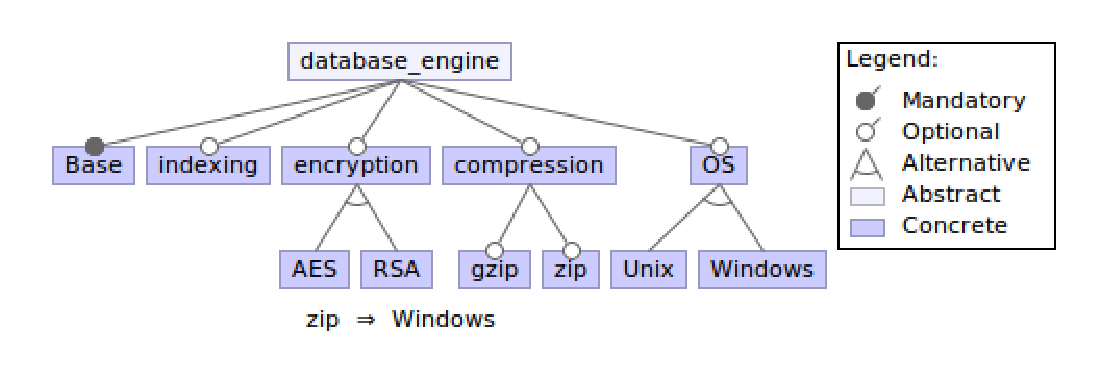
\includegraphics[width=0.8\textwidth]{images/example_database}
  \caption{Example database model (extended form section~\ref{background_conf_sys}).}
  \label{background_variab_models_feature_diagram_example}
\end{figure}

\subsection{Performance Assessment}
\label{background_perf}

The last section covers the introduction to Configurable Software Systems~(section~\ref{background_conf_sys}) and their representation through models~(section~\ref{background_variab_models}). 
This section concentrates on the term performance of configurable software systems. 
We define performance for this thesis~(section~\ref{background_perf}) and show how to assess performance to learn models from tested configurations. 
After that, we present approaches of how these models can predict performance.

\subsubsection{Performance in General}
\label{perf_general}

Performance is an important quality of software systems. 
As described in the introduction, definitions of performance differ depending on the perspective. 
The most used way is to explain performance of software as a non-functional property~\cite{Molyneaux:2009:AAP:1550832,liggesmeyer2002software}. 
They describe how a system provides its functionality. 
In contrast to that, there are functional properties which describe what a system should do. 
To decide if a system performs well, non-functional properties are compared to so called \acp{NFR}. 
They constitute a set of requirements which the software should fulfil. 
\acp{NFR} should be defined before the software is tested. 
Each type of a software system has different metrics which should be analysed. 
For example, a webserver can be analysed through the following metrics:

\begin{description}
	\item [Hit Rate] is the total number of requests arriving at a server in a defined time frame.
	\item [Latency] describes the time that has passed from the start of a request message until the response message starts being received.
	\item [Response Time] describes the time that has passed from the start of a request message until the whole response message is received.
	\item [Availability] describes the time that the software is available to the user.
\end{description}

With client-server applications, communication takes place through networks, whereas with off-line applications, the focus during the analysis of performance metrics lies on the intrinsic properties.
Off-line applications usually run on a single device and do not need to communicate direct with other systems. 
The following are some performance metrics of off-line applications:

\begin{description}
	\item [Resource Utilization] describes the fraction to which a system uses its resources\footnote{A resource is a system element that offers some service to other system elements that require them. Resources can be categorized into hardware components(CPU, bus, storage), logical elements(buffers, locks, semaphores) and processing resources (processes, threads)\cite{woodside2007future}.}.
	\item [Response Time] describes the time that is needed to complete an operation.
	\item [Throughput] is the amount of work done in a defined time.
	\item [Availability] describes the time that the software is available to the user.
	\item [Scalability] describes the ability to grow and perform an increasing amount of work. 
\end{description}

For this thesis, we will focus on off-line systems because we do not want to cope with the measurement inaccuracy which might accompany with the hardware and software of networks resources. 
Furthermore, we want to define performance as the amount of work done per unit of time~\ref{def:perf1} like~\cite{tsirogiannis2010analyzing}. 
So performance can be defines as:
\begin{equation}
	\label{def:perf1}
	\mbox{Performance}=\frac{\mbox{Work Done}}{\mbox{Execution Time}}
\end{equation}

Because we want to analyse performance of configurable software systems, we execute different variants of them using the same inputs (Benchmarks\footnote{Benchmarking is the process of running software with standardized tests to be able to compare the results and assess their relative performance.}) for all configurations. 
Thereby, we are able to compare them and since the \textsf{work done} is always the same, we are able to concretize our formula like~\cite{siegmund2015performance}:

%Because we want to analyze performance of software by executing benchmarks, the work done is always the same. So for this thesis we can define performance like~\cite{siegmund2015performance}:
\begin{equation}
	\label{def:perf2}
	\mbox{Performance}=\mbox{Execution Time}
\end{equation}

To identify performance hot-spots, we also acquire the run-time of each method which is executed.
We are interested in the time spent in each method (net-time).
The concrete approach is explained in section~\ref{perf_measure}. 


\subsubsection{\ac{SPE}}

After defining performance in general, we outline the process of analysing performance of software systems.
The process of analysing performance of software systems is defined as follows:
\begin{quote}
``\ac{SPE} represents the entire collection of software engineering activities and related analyses used throughout the software development cycle, which are directed to meeting performance requirements.''~\cite{woodside2007future}.
\end{quote}
There are two general approaches in literature~\cite{woodside2007future}: \textit{measurement-based} and \textit{model-based}. 
The model-based approach is applied early in the development cycle. 
It tries to create performance models to adjust design and architecture as early as possible. 
The measurement-base approach is applied late in the development cycle, because it will run tests and diagnosis to tune the software.
The whole process of \ac{SPE} activities can be structured into six parts. 
The first identifies the \ac{NFR} which should be analysed. In section~\ref{perf_general}, we sum up the important parts. 
Defining and analysing the requirements is the second step~\cite{woodside2007future}. 
This includes to specify the environment in which the software runs. 
For the sake of reproducibility, the environment should be defined carefully.  
To select specific tasks, there are many different benchmarks available (\href{https://bapco.com/}{BAPCo}, \href{https://www.eembc.org/}{EEMBC}, \href{http://www.spec.org/}{SPEC}). 
These and other benchmarks provide the possibility to compare one software product to another with a set of standardized tasks and workloads. 
Another possibility is to use benchmarks which are provided by the software itself. 
This may enable analysis of all functionality of software if the provided benchmarks are selected carefully. 
The third activity is to design models which predict performance from detailed design, architecture and usage scenarios. 
These models describe how systems use resources and how resource contention affects operation. 
These models are able to predict system properties before they are implemented to gather knowledge as early as possible in the software development live cycle.
The next \ac{SPE} activity is performance testing. 
Tests can cover only parts or the entire software, depending on the selected benchmarks. 
Here we get actual values for the performance metrics we selected.
From the gathered data, we can learn models to predict the effect of changes to the system, which is the fifth step of \ac{SPE}. 
A lot of effort has been spent in the last years to understand and improve performance. 
Section~\ref{rel_perf_pred} summarizes more recent measurement-based performance prediction approaches which emphasize variability.
The last step of \ac{SPE} is to analyse the total system.
Here the final deployed system is analysed regarding to the defined performance goals.

This thesis identifies concerns, defines and analyses requirements, conducts performance tests and learns models for performance prediction of configurable software systems. Because we follow the \textit{measurement-based} approach, we also evaluate the impact of the measurement environment. 


\section{Related Work}
\label{rel_work}

While the last section describes the necessary background for configurable software systems, performance and \ac{SPE}, this section deals with the topics performance prediction and performance analysis of Java projects. The first part deals with different approaches on learning the influence of feature selection on performance and presents different sampling strategies. The second part utilizes existing performance analysis tools.

% Performance in software systems
\subsection{Performance Prediction}
\label{rel_perf_pred}

The task of learning and predicting performance is subject of research for several years. Since then, several measurement-based performance prediction models were developed. In general, they all work the same way. They sample a subset of configurations because measuring performance of each configuration is not practicable if the configuration space is to big. They split the available measurements into two sets (learning set and test set). For learning a model, they use the learning set and to be able to assess the accuracy of the model they compare the test set with the prediction of the model. In the following, we describe the differences of some models.

One task of \acp{SPL} is to verify the large number of possible products. \cite{thum2012family} presented the approach, called family-based verification, in which the whole \ac{SPL} is encoded in a single \textit{meta-product} which simulates the behaviour of all individual products of the product line. The idea is to verify only the generated meta-product. It contains the implementation and specification of every feature. So, it is able to simulate each product. They verify the meta-product (family-based) instead of verifying all products separately (product-based). Because of the generation of the meta-product, they do not have different products from a product line, but a single system, so they are able to use the single-system theorem prover KeY for verification. They adapted the product simulator introduced by~\cite{apel2011detection} to translate the Java-based product line into the meta-product. In comparison to the product-based approach, the authors were able to save more than 85\% of the verification effort.

In contrast to that,~\cite{guo2013variability} presented an approach about learning the influence of feature selection on performance. The authors want to use few samples (linear in the number of features) to show that this is enough to learn performance behaviour. They make use of \ac{CART} to recursively partition the sample into smaller segments. The algorithm searches the available set of measurements according to the highest reduction of the cost function (squared error) and picks the best for the split. Each subset is then searched again until they can represent the current example set well enough with the tree. After that, \ac{CART} iteratively adds new samples and recomputes the algorithm to increase the overall prediction accuracy.

\cite{siegmund2012spl} presented an holistic approach, \textit{SPLConqueror}, to optimize learning the influences of features on \ac{NFP}. They automate the process of learning the influence of feature selection on performance, including sampling, measurement and creation of performance influence models. The authors want to find the optimal variant for \ac{NFR} by measuring the \acp{NFP} from a sample of all variants. They propose classification of \ac{NFP} resulting in two different measurement techniques: feature-wise (e.g. assessing performance of features) and variant-wise (e.g. assessing footprint of variants). They also introduce two sampling strategies to analyse the influence of individual as well as the influence of feature interactions of the sample. With \textit{feature-wise} sampling the influence of individual features \textit{f} to \acp{NFP} is analysed by sampling two variants of each feature. The first variant selects feature \textit{f} and the other variant deselects feature \textit{f}. Furthermore, as many other features as possible are not selected. So the difference between these two variants present the impact of feature \textit{f} on the \ac{NFP}. The other sampling strategy (\textit{pair-wise} sampling) works similar but uses each combination of two features.

A further development of the idea of how to build performance-influence models was introduced by \cite{siegmund2015performance}. They expand the tool \textit{SPLConqueror} to create simple, human understandable simple models with few measurements. Therefore, they applied different binary (e.g. Pair-Wise, Option-Wise, Negative Option-Wise) and numerical (e.g. Placket-Burman Design) sampling strategies\footnote{We will give an overview of sampling strategies in section \ref{perf_measure_sampling}.} and combined them. With these sample set they measured the performance of their subject systems to get inputs for the stepwise linear regression model. Measured performance serves as dependent variable and configuration options as independent. Linear regression tries to fit a line through measurement points by adjusting regression coefficients so that the global error is minimal. This approach incremental adds new regression terms to the formula in each round until a certain accuracy is reached or improvement in accuracy become marginal.

\cite{sarkar2015cost} proposed another approach to further reduce the number of samples needed to learn the influence of feature selection on performance. The authors wants to determine an ideal sample dynamically, that yield a good prediction accuracy with low measurement effort. They investigate two sampling strategies (projective sampling and progressive sampling) which both are used in data mining to reduce the size of data needed. After sampling, they used \ac{CART} like~\cite{guo2013variability} to calculate the prediction accuracy. A typically prediction model evaluation criteria is prediction accuracy, but \cite{sarkar2015cost} use an accumulated cost function consisting of (weighted) prediction error and costs for creation of test and training sets. With their approach they are able to reduce the number of elements needed for an initial sample. 

All aforementioned approaches rely on improving certain aspects of configurable software systems (or \acp{SPL}) modelling. They provide new strategies for sampling or present tools. The approach from \cite{thum2012family} reduces validation time of \acp{SPL} by 85\% for their case study. But this approach is only reliable if the configuration space is small enough. The \ac{CART}-Tool combines binary and numerical sampling with help of a simple and fast regression-tree approach. \cite{sarkar2015cost} further improves the size of necessary samples through projective sampling. But with the drawback that this strategy only works well with an proper initial sample. Finally the tool \textit{SPLConqueror} developed by \cite{siegmund2012spl} combines all aspects of \acp{NFP}-analysis including predefined sampling strategies, performance (and other \acp{NFP}) model learning and prediction with the implemented strategies. 

\subsection{Performance Analysis of Java Projects}
\label{rel_perf_java}

To the best of our knowledge there exist not work presenting how to model and predict performance on method level with Java projects. The initial research about this topic nevertheless revealed existing tools related to this topic. 

\cite{vanHoorn2012kieker} present a framework, ``Kieker'', for monitoring and analyzing the runtime behaviour of software systems. They want to monitor runtime behaviour of concurrent and distributed applications. Their tool is able to collect collecting timing and tracing information as well as sampling system-level measurements (CPE utilization and memory usage). ``Kieker'' also provides logging and streaming mechanism to save the data for later analysis or to visualisation incoming records direct. The tool also achieves an average monitoring overhead about of 10\% and is recommended by the SPEC Research Group.

Another tool which instruments Java is ``SPASS-meter'' introduced by~\cite{eichelber12spassmeter}. Like the framework of \cite{vanHoorn2012kieker} it instruments Java bytecode to profile \acp{NFP} like throughput or response time. It is also capable of logging CPU-usage of the \ac{JVM} or memory usage. The monitoring overhead which accompanies with instrumentation is comparable to that of ``Kieker''. Also memory overhead caused logging the measurements is not much different. 

The list of performance monitoring and analysis frameworks is not complete. We wanted to focus on open source tool which approached recently to motivate our decision on providing additional support in the field of configurability aware performance analysis of software systems. ``Kieker'' as well as ``SPASS-meter'' for example did not support handling high configurable software systems in combination with variability modelling and \ac{NFP} prediction.